\section{Evaluation} \label{sec:methods_evaluation}\label{app:evaluation}

\subsection{Test scores} We evaluate our agents on a suite of 1000 held out test tasks  sampled from the same distribution as the training games, using held-out world topologies. The procedure for pre-generating the XLand task pool is detailed in Appendix \ref{app:presample_tasks}. Rejection sampling ensures that no game (goal and production rules) in the test set is contained in the training set.

In XLand, rewards are obtained on every frame in which a goal is satisfied, making total rewards incomparable between tasks. To account for this, we fine-tune AdA on the test-task set. We compute the fine-tuned agent's maximum total last-trial reward
(over any number of trials up to 13)
and use this as an estimate of the maximum possible reward obtainable in a single trial of each test task. We call this quantity the normaliser. We define the \textit{test score} $S^i_m$ of an agent $i$ on task $m$ with $k$ trials to be the total reward obtained in trial $k$ divided by the normaliser. This normalises rewards roughly to the interval $[0, 1]$. Note that it is possible for an agent under evaluation to obtain a score greater than 1, both due to noise in the evaluation process and the fact that the agent under evaluation may be better than the one used for creating the normaliser.

When reporting the scores of our agents on a game with $k$ trials, we always use the total reward of the last trial. This is a good measure of whether the agent has successfully navigated the exploration-exploitation tradeoff in a novel MDP, given knowledge of the number of trials $k$. If an agent is capable of adaptation, we expect to see the performance in the last ($k$\textsuperscript{th}) trial increase as a function of $k$: that is to say, the agent is able to make use of additional experience on-the-fly to perform better. We evaluate on $k \in \{1, 2, 3, 5, 8, 13\}$, where $8$ and $13$ are held out values of $k$ that were not seen during training.

To aggregate the scores of an agent across games, we use a fixed (usually 20\textsuperscript{th}) percentile score \citep{DBLP:journals/corr/abs-2108-13264}. This gives us a lower bound guarantee on the performance of the agent across most of the tasks: for example, if the 20\textsuperscript{th} percentile score of an agent is $0.5$, then the agent gets the score of at least $0.5$ on $80\%$ of the games. Using an aggregation method like this (as opposed to an average) allows us to concentrate on the coverage of many tasks, as opposed to focusing the effort on improving the performance on outlier tasks. Empirically, we find that our results are robust across a range of different percentiles. 

\subsection{Hand-authored probe tasks} 
Evaluation using test tasks can only give us information with respect to the pre-sampled distribution in Appendix \ref{app:presample_tasks}. While this is certainly vast and diverse, an arbitrary task sampled from the test set is not necessarily easily understandable for humans. So in addition to quantitative evaluation on $1000$ test tasks we also investigate specific human-level capabilities of our agent on two sets of $30$ single-agent and $28$ multi-agent probe tasks. These are based on situations that are intuitive to humans and which require qualitatively different behaviours, which we can inspect in more detail ``with the naked eye''. A full description of all $58$ probe tasks can be found in Appendix \ref{appendix:human_scale_adaptation}. Representative single-agent and multi-agent probe tasks are described in detail in Figures \labelcref{fig:wrong-pair-disappears-explained,fig:pyramid-in-a-haystack-explained,fig:no-touchy-explained}.

\subsection{Adaptation metric} 

We introduce an \textit{adaptation metric} to rank our agents based on their few-shot adaptation capability across the hand-authored probe task set. We collect last-trial total reward for all $(m, k)$ pairs where $m$ is a probe task and $k \in \{1, 2, 3, 5, 8, 13\}$. We normalise the per-task scores just as for the test set above. We then aggregate over tasks using the $50$\textsuperscript{th} percentile (median). Finally, we aggregate over $k$ by saying that agent $A$ ranks higher than agent $B$ if and only if $A$'s task-aggregated scores are a Pareto improvement over $B$'s. That is to say, we would like agents that are both capable of high-quality zero-shot generalisation where possible ($k = 1$), and also that can use additional trial information to efficiently improve their policy in few-shots $k > 1$; we don't ``trade-off'' between these. 

A convenient way of using the Pareto improvement criterion to compute a scalar metric is the Nash average method of \citet{balduzzi2018re}. We construct a competitive meta-game of ``agents vs. $k$'', and compute the maximum entropy Nash equilibrium for the game. The Nash payoff is then used as the adaptation metric, and agents are ranked by this metric. As desired, this metric has the property that if neither agent $A$ nor agent $B$ Pareto-dominate the other, the $A$ and $B$ receive the same Nash payoff and are therefore ranked equally. This adaptation metric was used as the means of selecting hyperparameters for training our best performing agent in Section \ref{sec:results_human_scale_adaptation}.

\begin{figure}
  \begin{minipage}[c]{0.65\textwidth}
        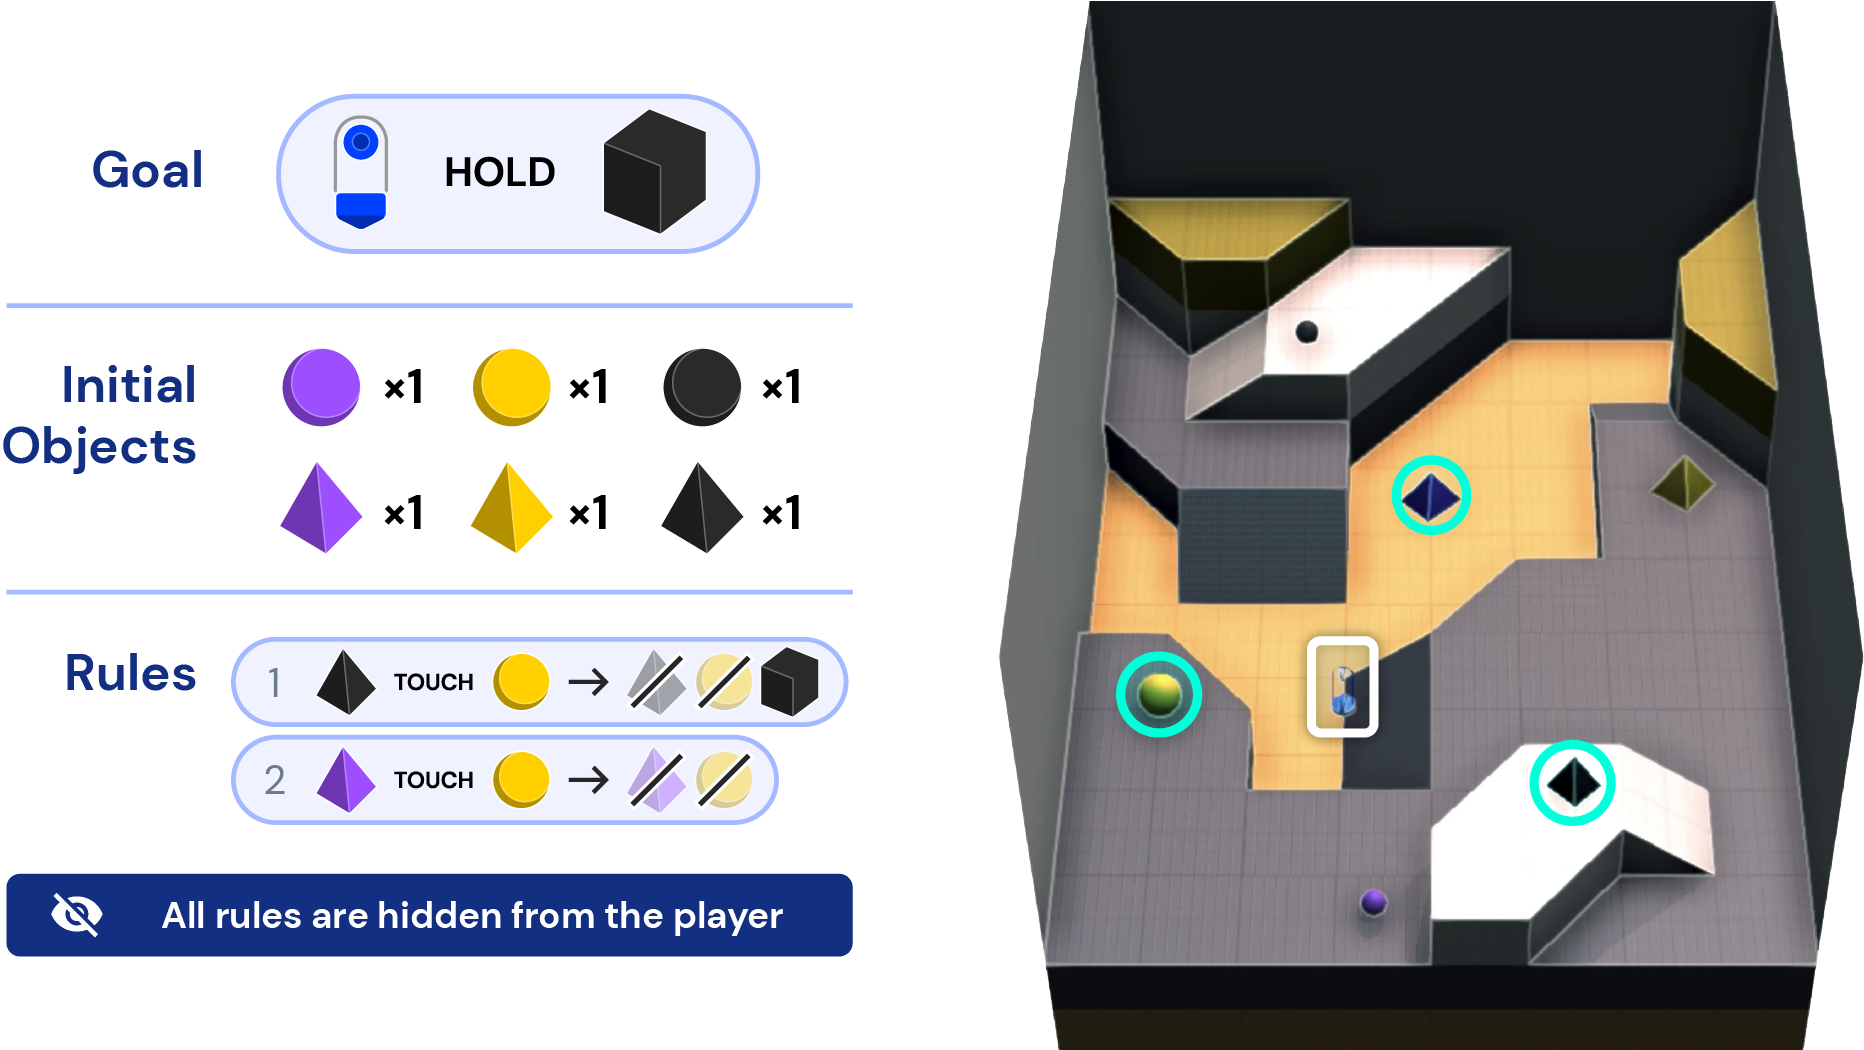
\includegraphics[width=1\textwidth]{figures/tasks/single-agent/wrong_pair_disappears_2.png}
  \end{minipage}\hfill
  \begin{minipage}[c]{0.3\textwidth}
    \caption{\textbf{Wrong Pair Disappears}: The player's goal is to hold a black cube, which does not exist among the initial objects. But there are two (hidden) production rules. The player needs to identify the correct world state which triggers the rule that creates the cube and not the one which destroys the necessary inputs. All this is embedded in a challenging world layout with one-way drops and limited visibility.} \label{fig:wrong-pair-disappears-explained}
  \end{minipage}
\end{figure}

\begin{figure}
  \begin{minipage}[c]{0.65\textwidth}
        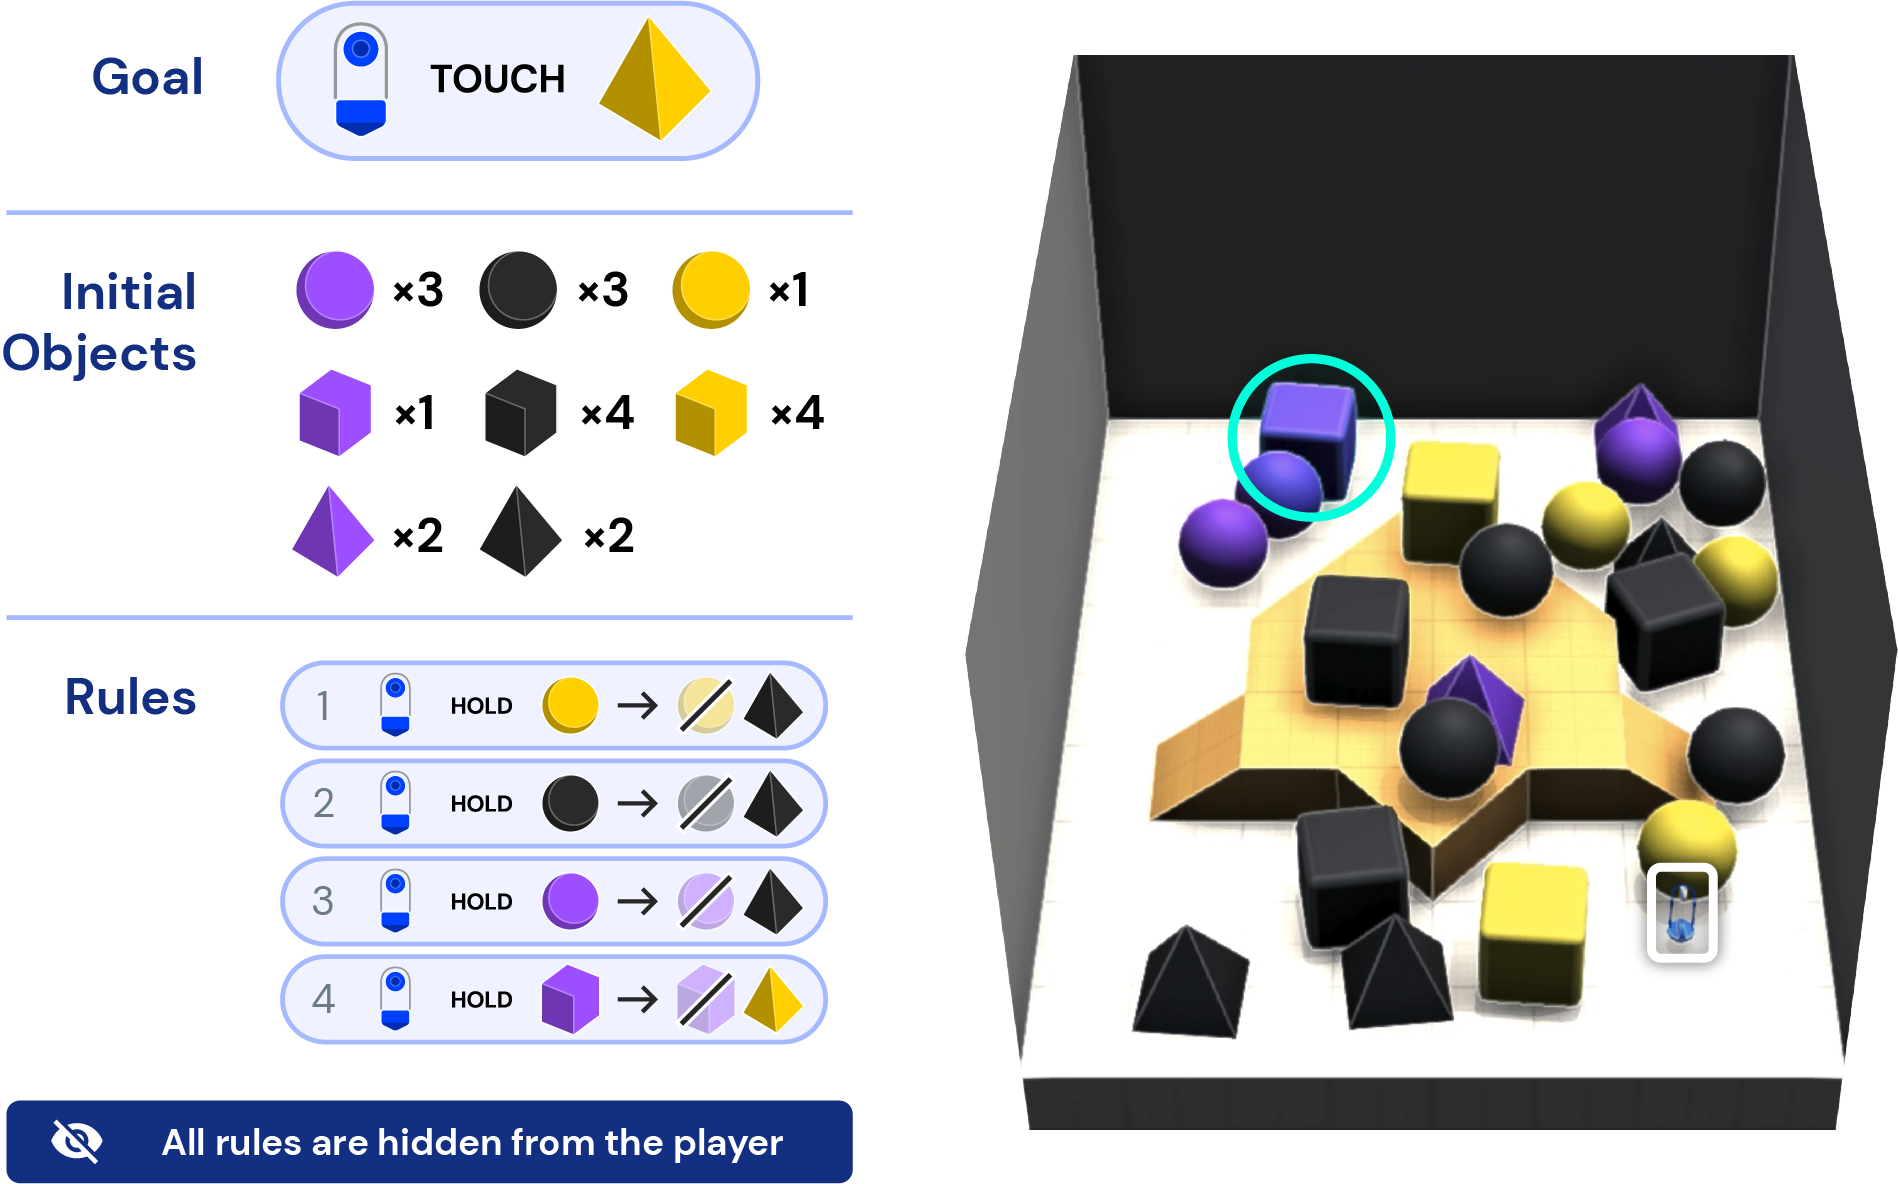
\includegraphics[width=1\textwidth]{figures/tasks/single-agent/pyramid_in_a_haystack_2.png}
  \end{minipage}\hfill
  \begin{minipage}[c]{0.3\textwidth}
    \caption{\textbf{Pyramid in a Haystack}: To create the necessary yellow pyramid, the player needs to find and hold the purple cube. There are several distractor objects and distractor rules in this world, requiring the player to deal not just with a hard exploration challenge but also a very noisy environment.} \label{fig:pyramid-in-a-haystack-explained}
  \end{minipage}
\end{figure}

\begin{figure}
  \begin{minipage}[c]{0.65\textwidth}
        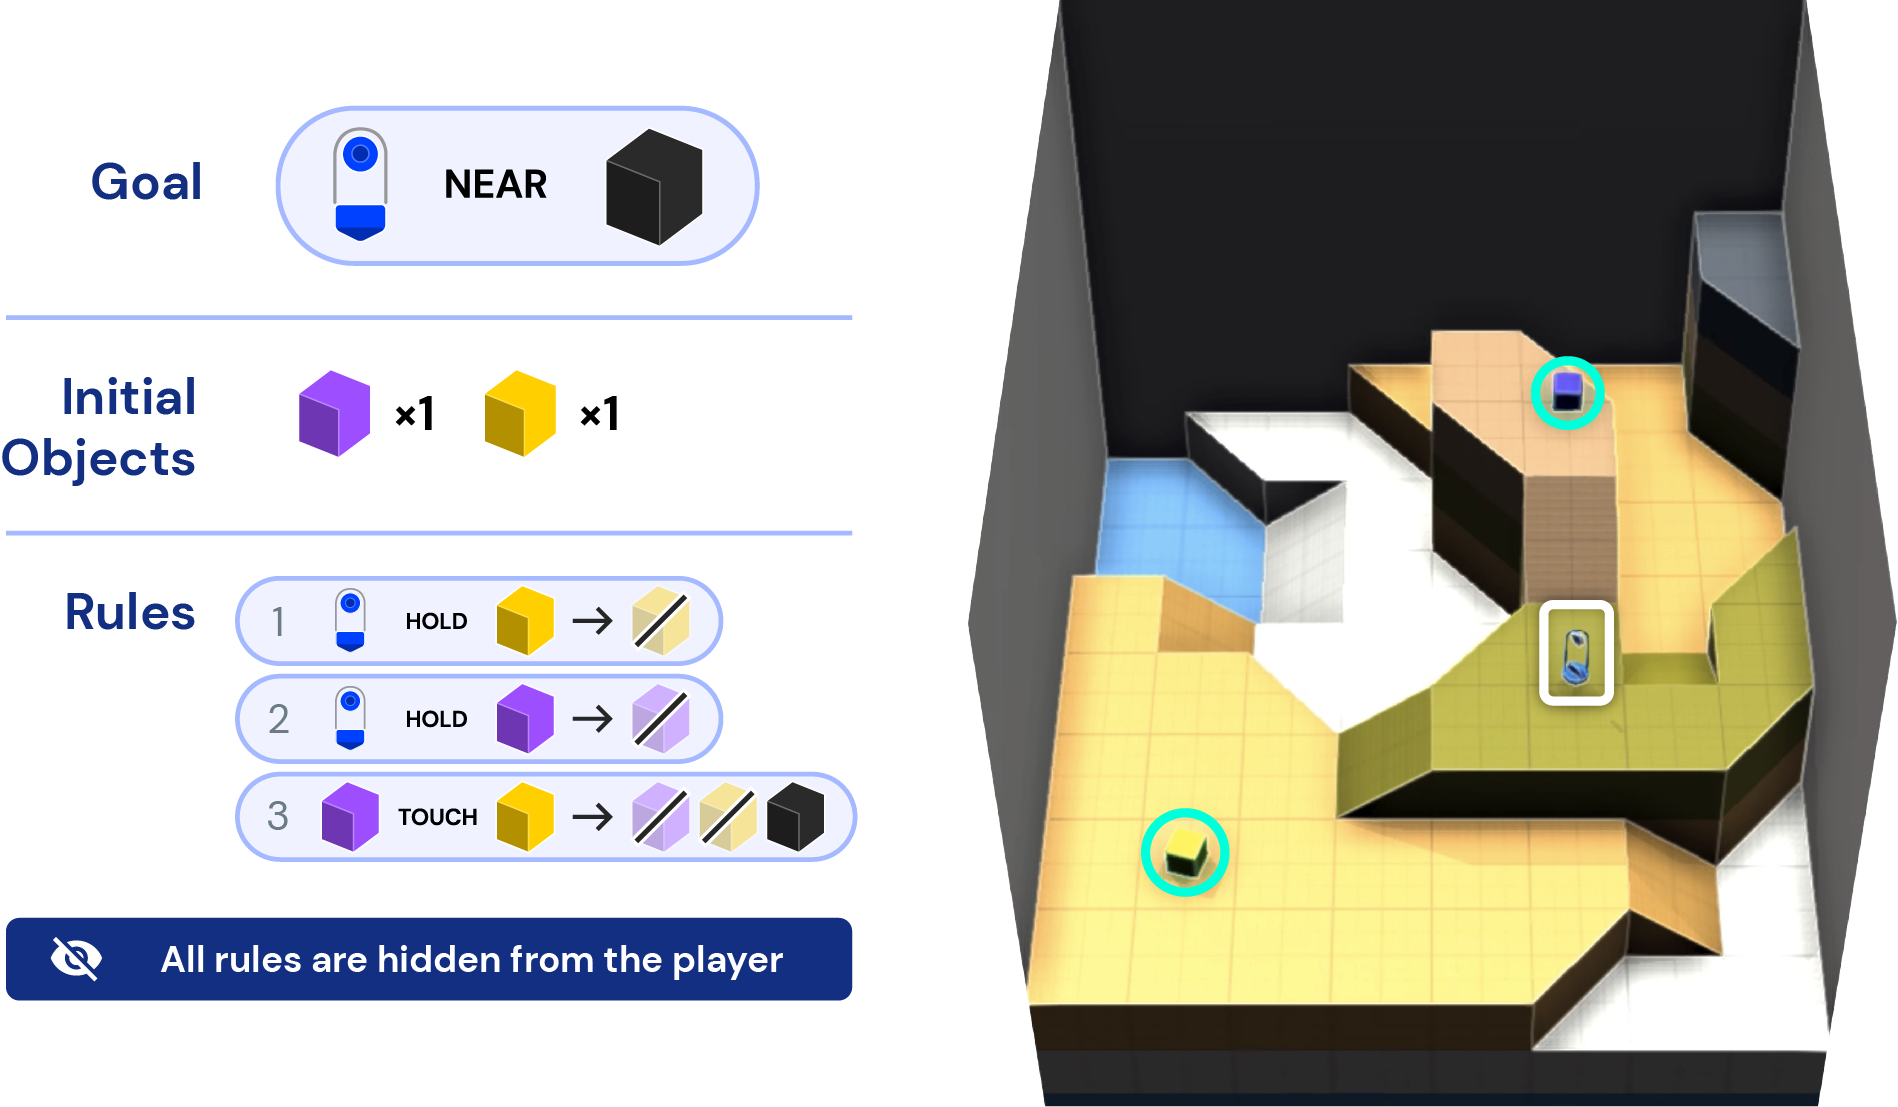
\includegraphics[width=1\textwidth]{figures/tasks/single-agent/push_dont_lift_2.png}
  \end{minipage}\hfill
  \begin{minipage}[c]{0.3\textwidth}
    \caption{\textbf{Push, don't lift}: The vast majority of training and evaluation tasks require lifting objects. Here two hidden rules destroy any object when lifted. In order to create the goal state, some ``lateral thinking'' is necessary: the player needs to identify that pushing the cubes with their body is possible.} \label{fig:no-touchy-explained}
  \end{minipage}
\end{figure}

\begin{figure}
  \begin{minipage}[c]{0.65\textwidth}
        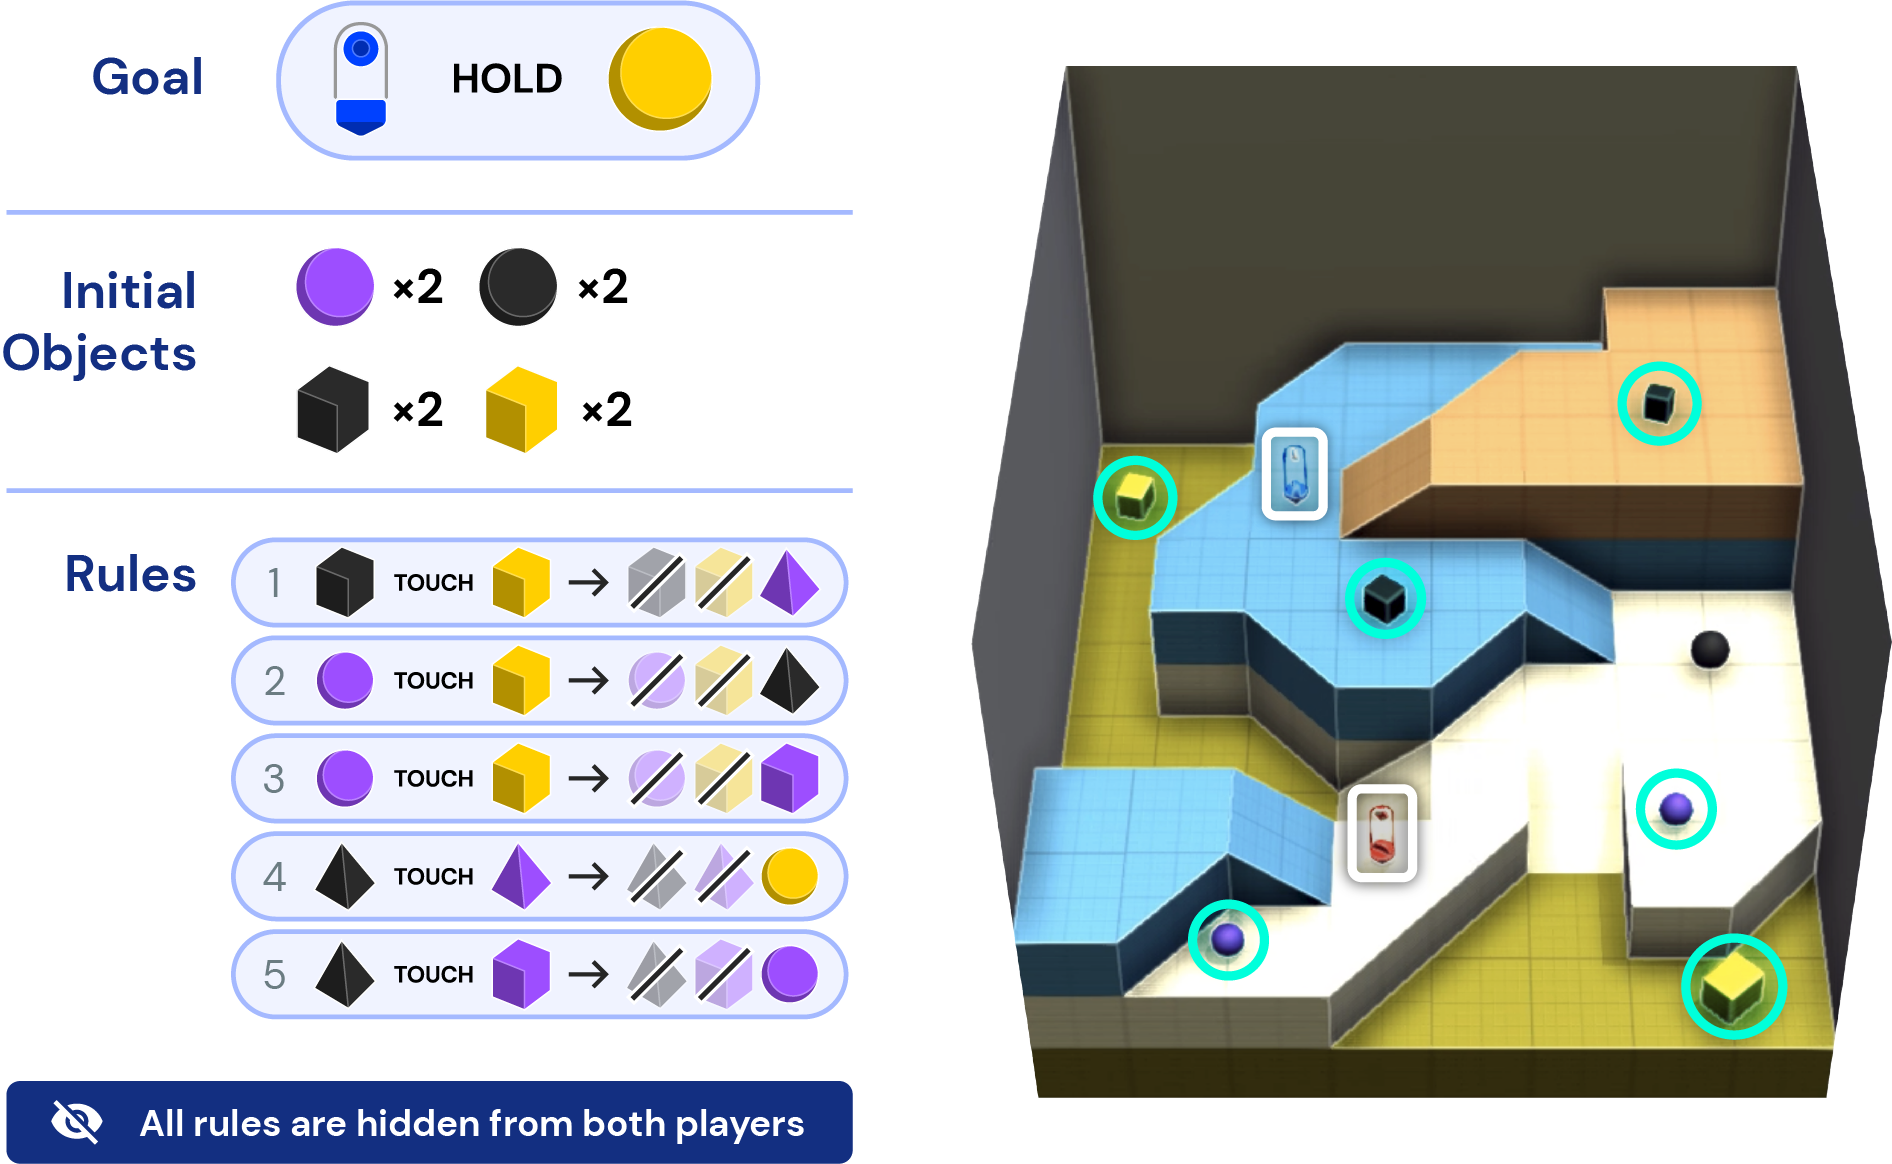
\includegraphics[width=1\textwidth]{figures/tasks/multi-agent/ma_irreversible_production_2.png}
  \end{minipage}\hfill
  \begin{minipage}[c]{0.3\textwidth}
    \caption{\textbf{Irreversible production for two}: Both players score when the first player holds a yellow sphere. There is no yellow sphere initially, but it can be produced from executing the first, second and fourth production rules in order. The other two rules are dead ends, destroying key input objects. Note that some input objects exist multiple times in the initial state, so there are multiple solution paths.} \label{fig:ma-irreversible-production-explained}
  \end{minipage}
\end{figure}

\subsection{Human data collection}\label{app:human-data-collection}

To provide a benchmark for human-timescale adaptation, we collected score data from a pool of $100$ human players on the $30$ single-agent probe tasks. Before attempting the probe tasks, each player completed a graded training curriculum of $23$ tasks to acquire familiarity with the mouse-and-keyboard control scheme and user interface (Figure \ref{fig:human_ui}), and the particular game mechanics of XLand. Since humans cannot undergo a short-term memory ``reset'' on episode boundaries, individual players attempted each of the probe tasks for a single $k$ only, with $k \in \{1, 2, 3, 5, 8\}$. All players experienced a variety of $k$ across the task set. We assigned each player a unique ordering of the $30$ probe tasks to average out any knowledge transfer from earlier tasks to later, and, within those orderings, we imposed separation between tasks with known similarity. Technical problems (e.g. internet dropout) prevented completion of 3.4\% of the $3000$ episodes, leaving an average of 19.3 samples per (task, $k$) pair, and a minimum of 17 samples for any individual (task, $k$).

\begin{figure}
    \centering
    \begin{subfigure}[b]{0.45\textwidth}
        \centering
        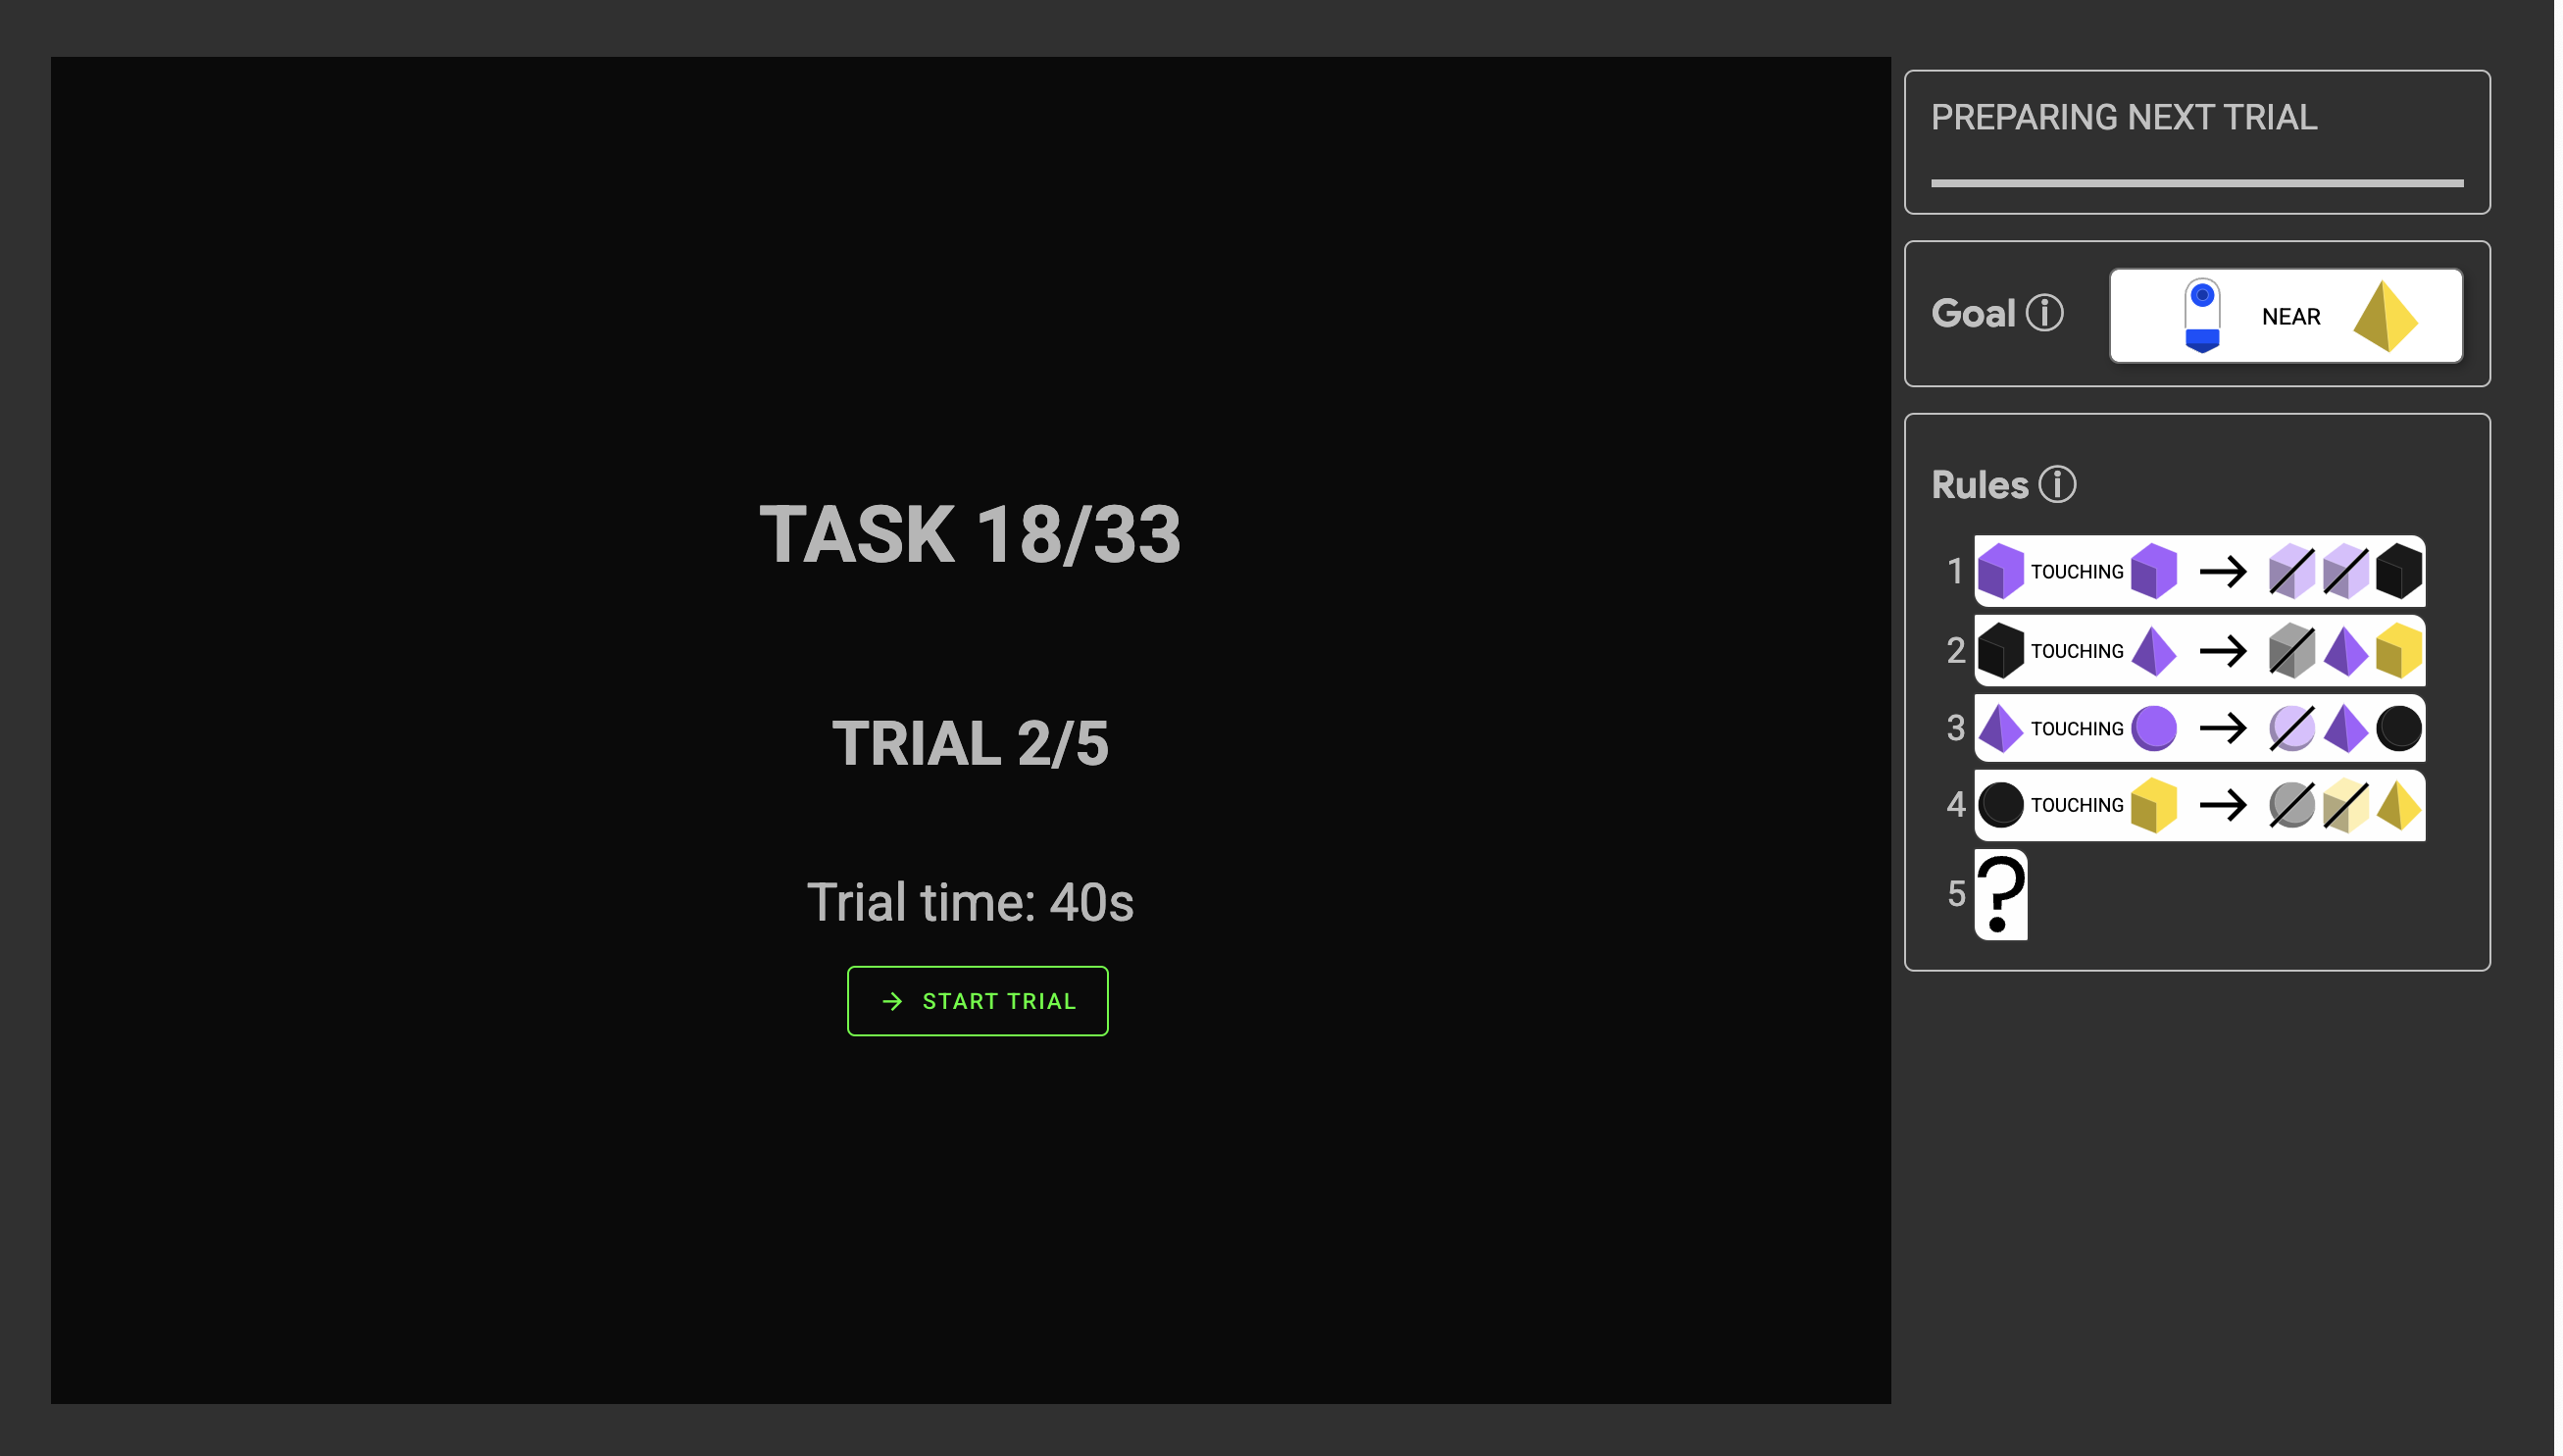
\includegraphics[width=\linewidth]{figures/human_data/human_ui_interstitial.png}
        \caption{}
    \end{subfigure}
    \begin{subfigure}[b]{0.46\textwidth}
        \centering
        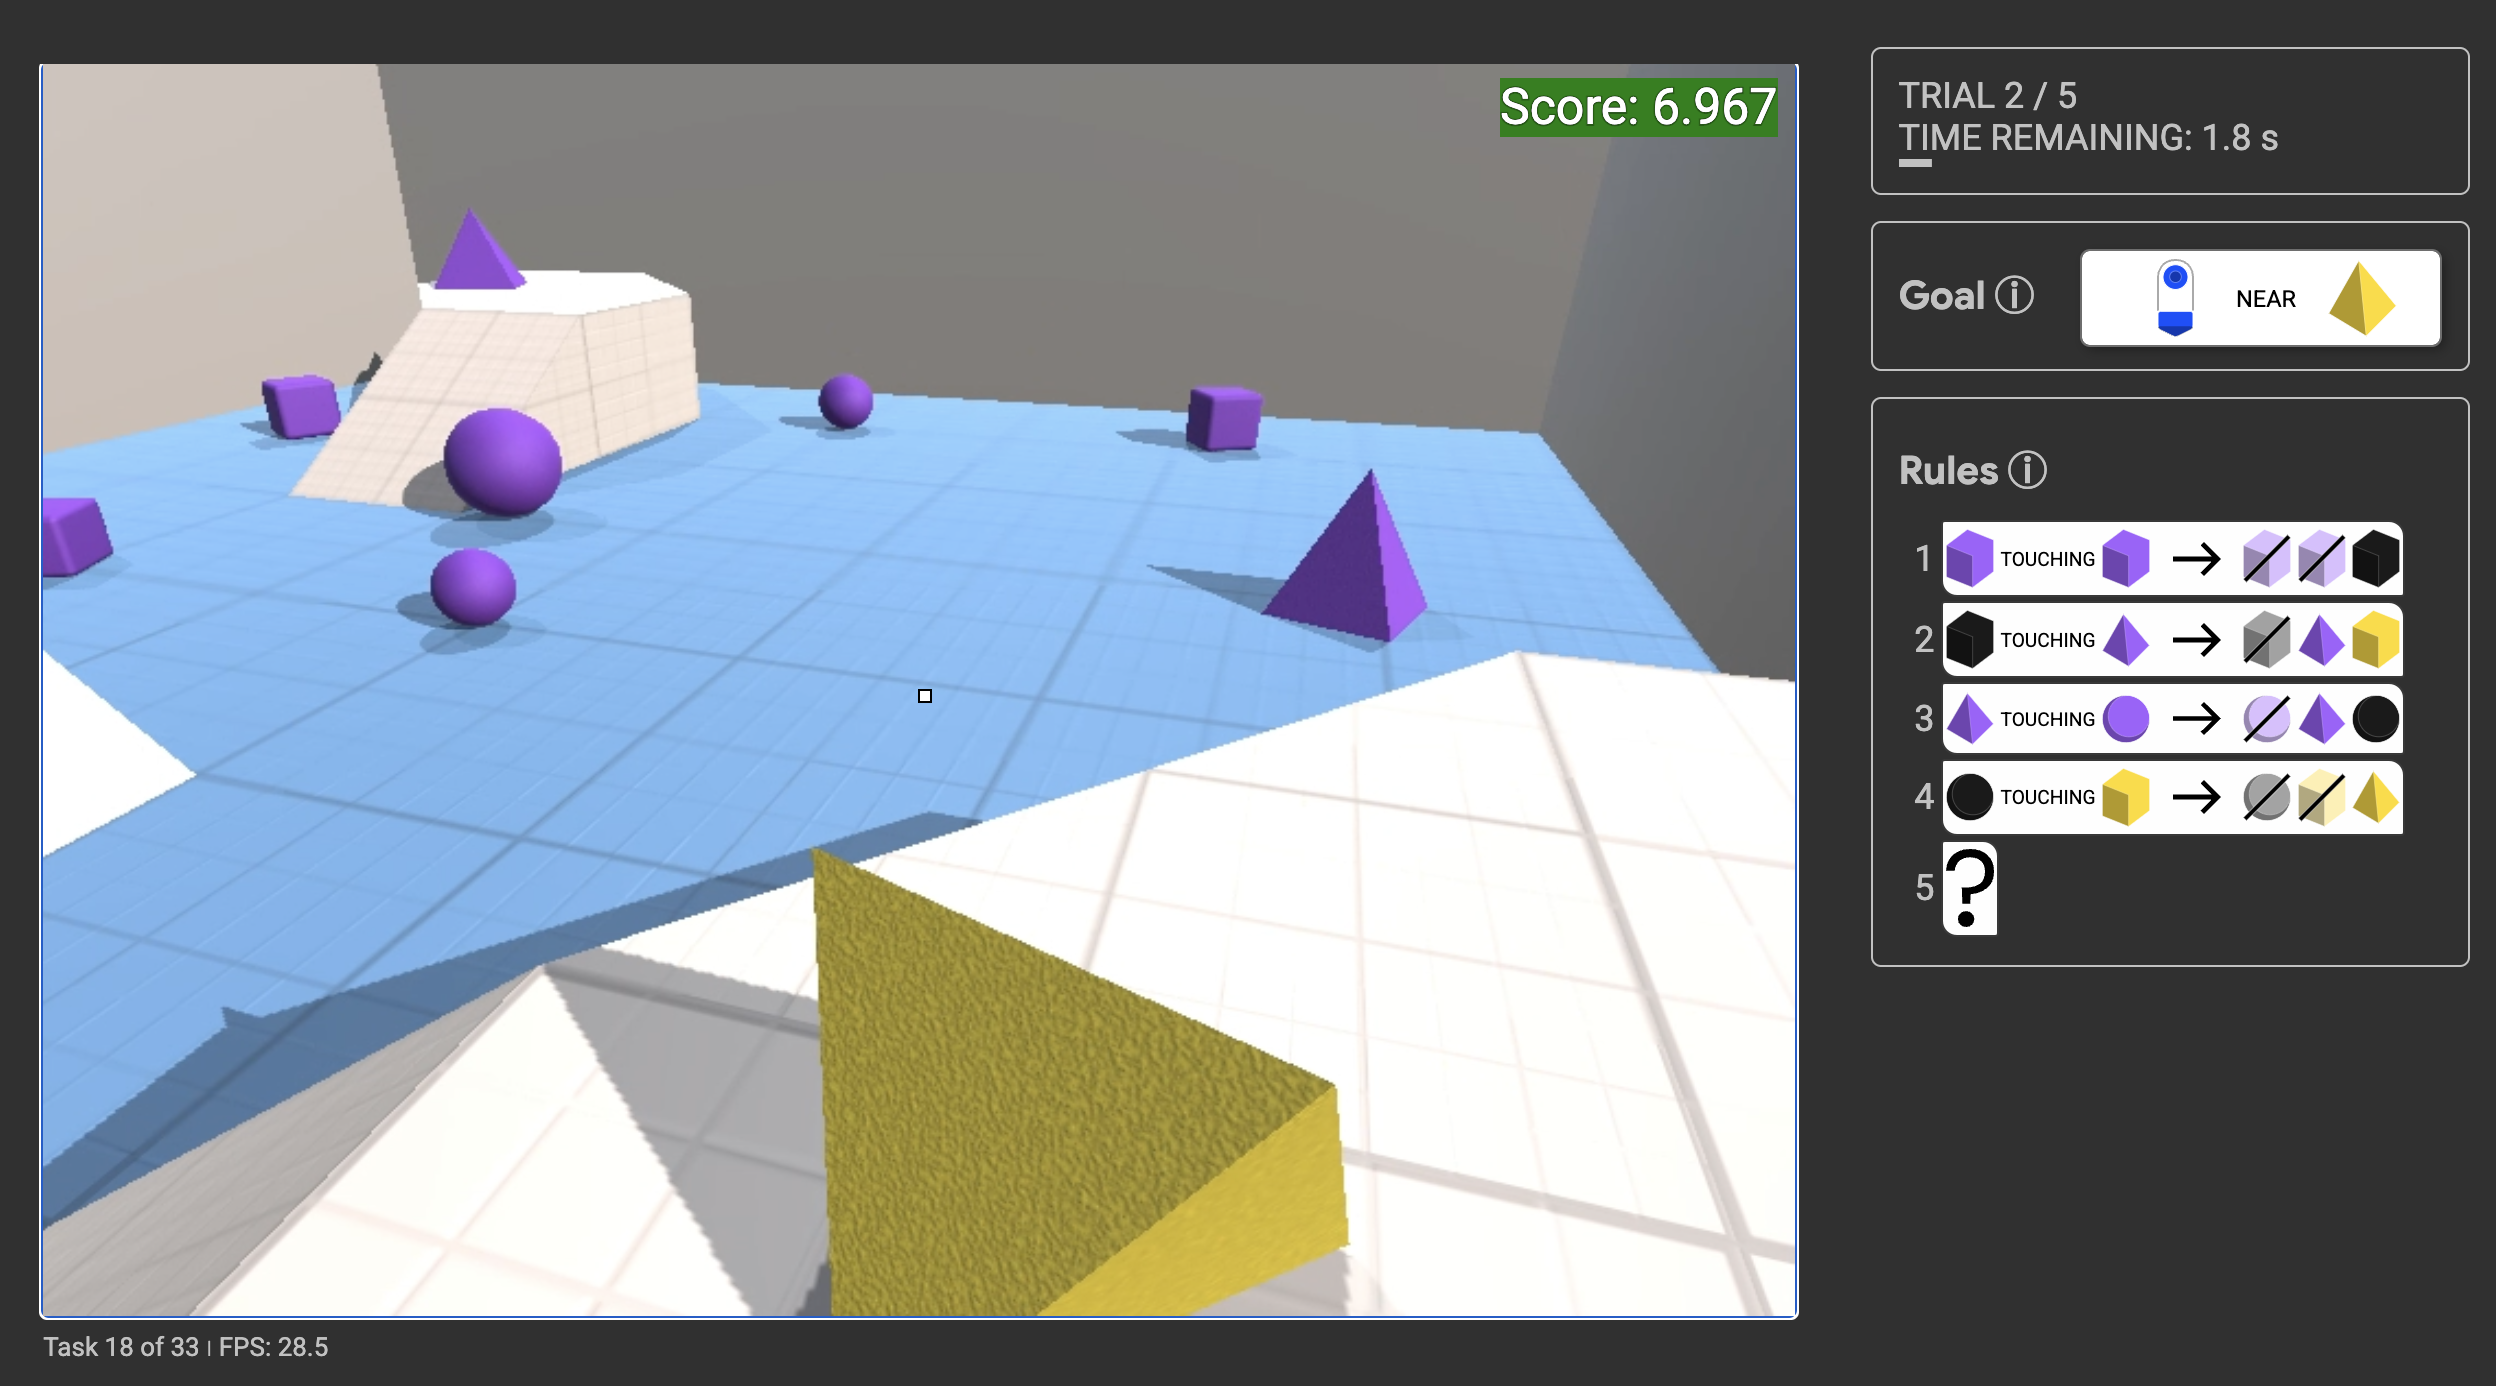
\includegraphics[width=\linewidth]{figures/human_data/human_ui_gameplay.png}
        \caption{}
    \end{subfigure}
\caption{The human player interface. \textbf{(a)} Prior to each trial players are told how many trials they have remaining on the current task, and are given unlimited time to read the goal and production rules (subject to any hiding). \textbf{(b)} During the trial players observe the same first-person camera view as agents, but at a higher $800 \times 600$ pixel resolution. The goal, production rules, current score, and time remaining in the trial are displayed via UI elements.}
    \label{fig:human_ui}
\end{figure}